\section{Application Android}

\subsection{Utilité}
Dans le but de pouvoir entraîner un modèle pour prédire le type de dégradations rencontrées sur la route de manière adéquate, il est nécessaire d'avoir un nombre important de données. C'est pourquoi rendre la collecte de données la plus pratique et efficace possible peut faciliter cette collecte et répondre à notre besoin.

Nous avons donc d'abord utilisé un robot équipé de deux cartes Arduino, mais nous avons pensé qu'il serait plus judicieux de mettre en place une application mobile qui permettrait d'effectuer la même tâche. En effet, l'idée d'utiliser une application mobile est de rendre la collecte de données accessible à toute autre personne munie d'un véhicule. L'utilisation de l'application nécessitera dans un premier temps des restrictions concernant la disposition du téléphone dans le véhicule (position, orientation, support utilisé). Cela permettra de diversifier les données et de les augmenter quantitativement, étant donné qu'il y aura un nombre important de collecteurs de données.

\subsection{Développement}
L'application actuelle sur laquelle nous travaillons a été codée en Kotlin et en Java à l'aide d'Android Studio qui est un environnement de développement pour développer des applications mobiles Android (Figure \ref{android_studio_2}). La présence de nombreux tutoriels mis en place par Android Studio, ainsi que de forums nous a permis d'avancer sur le développement du code.

\begin{figure}[htbp]
  \centering
  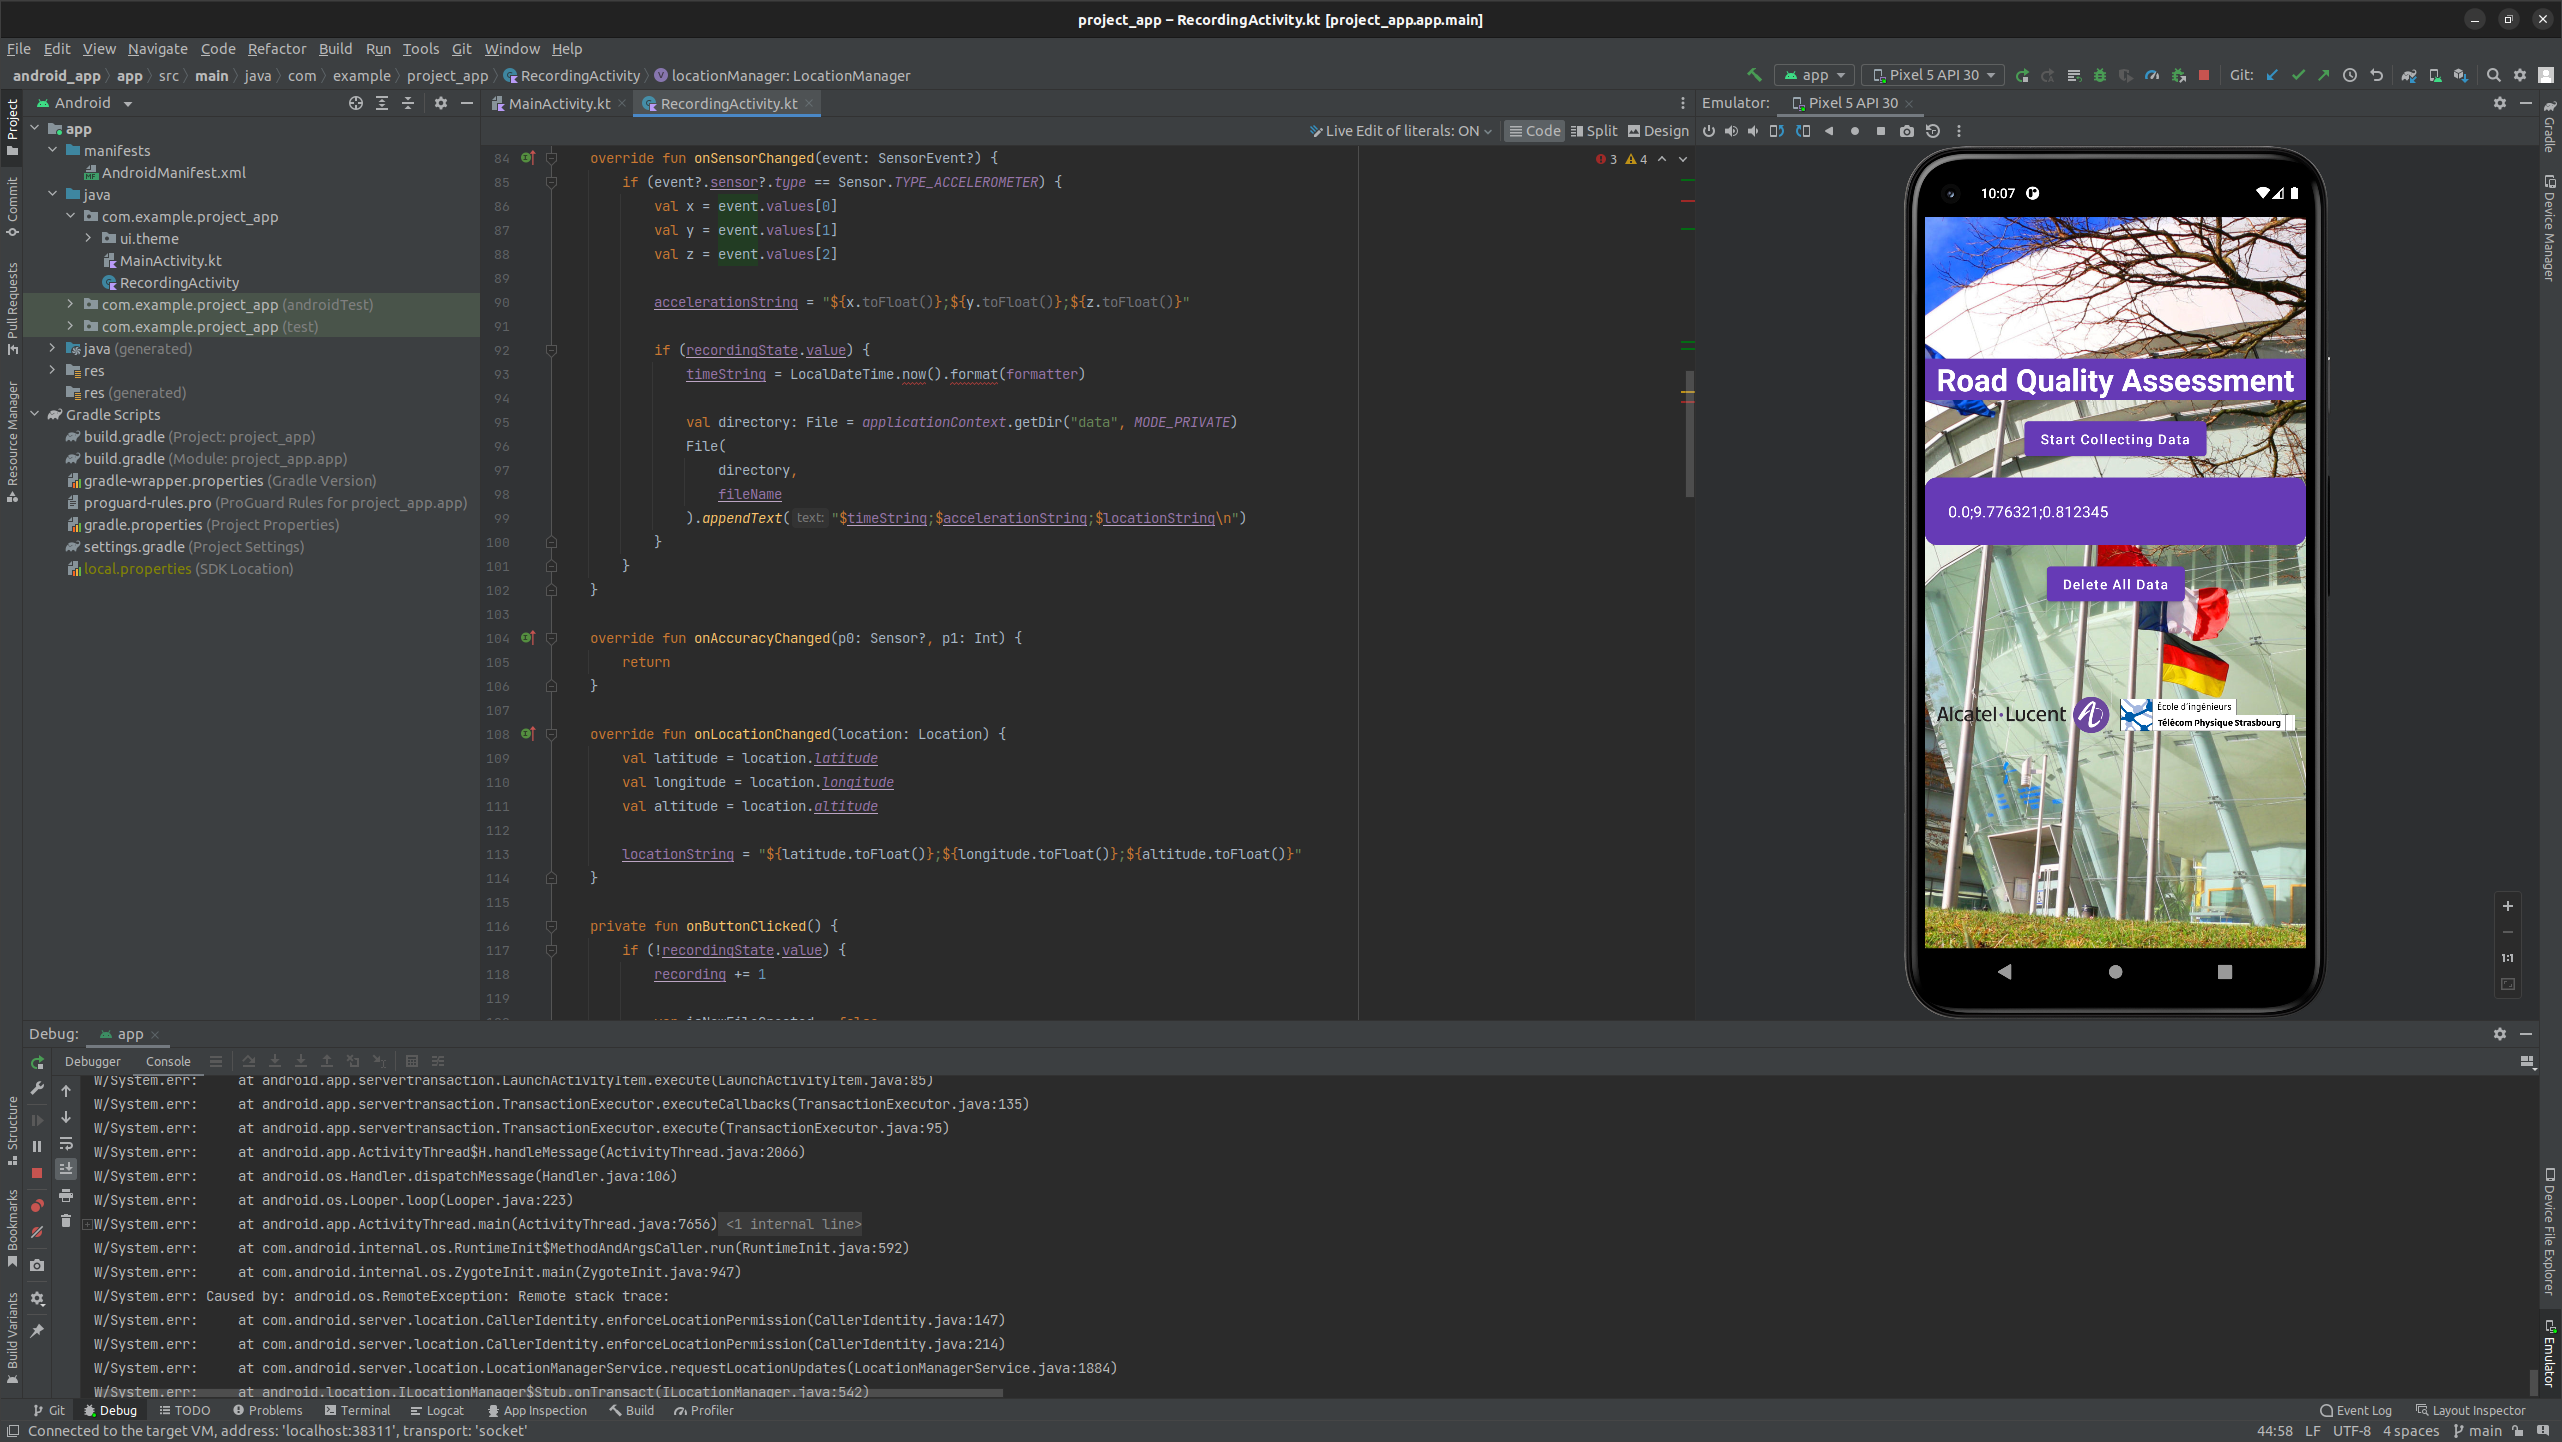
\includegraphics[width=0.8\textwidth]{img/android_studio_2.png}
  \caption{Capture d'écran d'Android Studio lors du développement de l'application}
  \label{android_studio_2}
\end{figure}

\subsection{État de l'application}
À l'heure actuelle, l'application est capable de collecter les données accélérométriques avec le \textit{timestamp}. Cependant, les enregistrements sont écrits dans des fichiers réservés à l'application, c'est à dire qui ne disponibles qu'en passant par Android Studio. Ce défaut rend donc la collecte de données non accessible pour tous les utilisateurs. Nous avons en revanche pu créer une seconde application avec Android Studio qui peut enregistrer les données GPS du téléphone, et cette fois-ci dans un fichier qui est accessible directement depuis le téléphone. La tâche en cours est donc d'implémenter cette particularité d'enregistrement de fichier dans l'application principale.

\subsection{Rôle futur envisagé}
Une fois que les problèmes d'enregistrement de fichiers seront résolus, la prochaine étape de l'application sera de la relier au modèle d'apprentissage que nous aurons mis en place, et de permettre ainsi de détecter et d'identifier le type de dégradation au moment même où la voiture se déplacera et rencontrera les détériorations de la route.